\chapter{Spin glasses}

Since spin glasses represent a huge field of study with a vast number of models, we will not define a spin glass in a general way.In this work we will refer to spin glasses only as Ising models with random interactions (that is in reality a really small subset of the studied spin glasses). 

In this chapter I will give a brief overview of the two most important models of spin glass, that are the Edwards-Anderson spin glass and the Sherrington-Kirkpatrick spin glass (also known as the mean field model). Then I will define the main object of our investigation: the Bethe lattice spin glass (BLSG), outlining the main features of such model.

\section{Main spin glass models}

We will call spin glass a collection of $N$ Ising spins $\sigma_i$, $(i=1,\dots,N)$, (an Ising spin is variable that can assume only two values, typically $\pm1$, $\sigma \in \{-1,1\}$) interacting only in couples with a magnitude for each link $J_{ij}$ extracted from a probability distribution $P_{ij}(J_{ij})$. A configuration is determined when every spin $\sigma$ has a determined value, hence we say that a configuration of the system is a string of Ising spins $C = \{\sigma_0,\sigma_1 \ldots, \sigma_N\}$. 
We
Each configuration $C$ has a Gibbs measure $\rho(C) \propto \exp(-\beta \mathcal{H[C]})$, with a Hamiltonian given by

\begin{equation}
\mathcal{H} = -\sum_{<ij>} J{ij} \sigma_i \sigma_j - \sum_i^N f_i \sigma_i
\end{equation}
The sum over $<ij>$ has to be intended as a sum over each possible couple $\sigma_i , \sigma_j$ connected by a link. The first term will be called the interaction term, the second one will be called the external term, and represents the action of an external field on the system. In the continuation of this work we will shut down the external field and set each $f_i=0$.

Spin glasses are a generalization of a very important model in statistical mechanics, called Ising model (IM). The original IM is obtained from our spin glass positioning every spin in a site of a bravais lattice and setting each $J_{ij}$ equal to one for nearest neighbors, and equal to zero otherwise.
A detailed investigation of the Ising model may be found in a vast collection of books ( \cite{stat} as good example, or \cite{huang} for an elementary introduction).
Let us summarize the main attributes of the Ising model.

\begin{itemize}
\item{A phase transition is present at finite temperature.}
\item{In the low temperature phase the system has a macroscopic magnetization.}
\item{The high temperature and the low temperature phases are very different: it is very easy to determine if at a give temperature we are in the high or low temperature phase (an exception is made for those temperatures near to the critical point.}
\item{The definition of an order parameter is straightforward as the magnetization.}
\item{The up/down symmetry is spontaneously broken in this phase (this is called SSB, spontaneuos symmetry breaking), system may be in one of two possible states at zero temperature.}

\end{itemize}

The main feature that distinguish spin glasses is the existence of a phase where the spins freeze in a complicated random configuration. Similar in some aspects, spin glasses behave very differently from Ising models

\begin{itemize}
\item{A new phase transition is present at finite temperature.}
\item{In the low temperature phase the system has not a definite magnetization. Total magnetization is zero, however each spin has a definite magnetization that is generally different from zero.}
\item{There are not two states in the low temperature phase. An infinite number of ground states appears. This complicated symmetry breaking is called replica symmetry breaking (RSB).}

\end{itemize}


Unlike ferromagnetic models, spin glasses may freeze in a huge number of different possible configurations. The term
This implies a nonzero entropy even at zero temperature (this is de facto a violation of the second principle of thermodynamics). Every configuration has no apparent order, the mean magnetization is zero in the glassy phase. Turns out that the classification of the glassy phase using an order parameter $q$ (such as magnetization in ordinary ferromagnets) fails. It is now well known that a good order parameter for the glassy phase involves an infinity of values and thus is a function $q = q(x)$. It would take a book to describe all the properties of spin glasses, so I will cut to the chase and send the willing reader to an opportune bibliography( \cite{beyond} and \cite{glass}).

\subsection{The replica method}

The replica method \cite{trick}(sometimes referred as replica trick \cite{critic})  is a mathematical method that takes advantage of a well known limit:

\begin{equation}
\log{ \mathcal{Z} } = \lim_{n\rightarrow 0} {  \mathcal{Z}^n - 1 \over n}
\label{tricky}
\end{equation}

When one has to average the free energy over each configuration of the disorder the limit \ref{tricky} comes in aid. Obviously performing $\langle F \rangle = \langle -\beta\log\mathcal{Z} \rangle$ is different from performing $  -\beta\log \langle\mathcal{Z} \rangle$, and the physics these two formulas reproduce is very different (the first is called quenched average, the second annealed average; the different meaning of these two types of averages is straightforward and well investigated in the major books of this field. A good introduction on this topic is found in \cite{glass}). In the spin glass problem we have to perform a quenched average. This physically means that each time we set a configuration of the disorder (each configuration differs from the others in the definition of each $J_{ij}$), it will not change during the evaluation of the observables (this is the reason of why one usually refers to frozen disorder). Roughly speaking, as the opposite case, when one performs an annealed average, the disorder acts as thermodynamic parameter, with the main effect of raising the effective temperature of the system.

When using \ref{tricky} we are able to trasform $\langle log\mathcal{Z} \rangle$ into $\langle \mathcal{Z}^n \rangle$. This means that we have now $n$ identical partition functions, and we have to evaluate every observable in this new n-times replicated system. At the end of the computations $n$ must be sent to zero, as the limit \ref{tricky} imposes.

The replica method is a powerful method for the study of the quenched disordered system, however the limit $n\rightarrow 0$ appears strangely defined. What we do is an analytic continuation to zero of a succession that is defined only on entire numbers. This passage is mathematically unprecise and usually a result obtained in the replica framework must be controlled using more stable methods.


\section{Two antipodal models}

\subsection{The Edwards Anderson model}

The most intuitive Ising spin glass is called the Edwards Anderson (EA) model. It consist in a collection of Ising variables $\sigma_i$, $\sigma = \{\pm 1\}$ organized in a regular lattice. Each interaction $J_{ij}$ between $\sigma_i$ and $\sigma_j$ is chosen random according to a given rule (which is typically a bimodal distribution).

The Hamiltonian of the system may be written as
\begin{equation}
\mathcal{H} = \sum_{<ij>} J_{ij}\sigma_i\sigma_j + \sum_i H_i \sigma_i
\end{equation}

This model has an equilibrium solution available in one dimension \cite{medina}. It predicts the existence of metastable states and gives a simple qualitative explaination of the slow off-equilibrium dynamic of spin glasses.

A large number of numerical investigations (as an example: \cite{EA}) has been made on the EA spin glass. This model exibiths all the major features of spin glasses, such as the spin glass phase transition, scale free relaxation and phase democracy. Particular remark must be made on the fact that slow relaxation poses a challenging point on the simulation of spin glasses in the low temperature phase. A number of
interesting methods has born to overcome this problem; as an interesting example I would cite the multispin coding technique \cite{multispin}, which allows to gain a factor of 50 in the simulations time. The authors of \cite{multispin} arrived to an astounishing performance of 33.5 picoseconds per single spin flip.

Though conceptually very simple, the EA spin glass represents a very difficult statistical mechanics problem.

\begin{figure}[h]
\centering
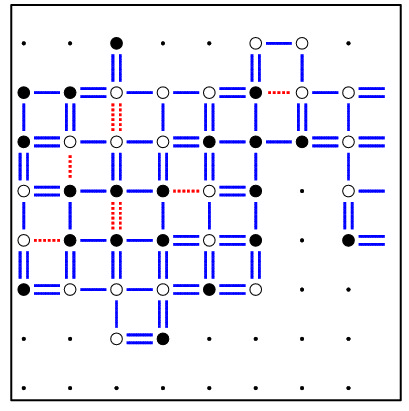
\includegraphics[scale =0.6]{img/edwards.jpg}
\caption{A representation of a 2D Edwards Anderson spin glass}
\label{fig:EA}
\end{figure}

 The EA model has been studied both with bimodal link distribution and Gaussian distribution. In fact, restricting on these two link distributions is typical in the spin glass problem. We recall that the bimodal link distribution is the one where each $J_{ij}$ is chosen from a set of two values (typically $\{\pm 1\}$), while the Gaussian link distribution is the one which has a probability density function for each link that is Gaussian. The major efforts of the analytical studies on EA model verted on the proprieties of the ground state of the system \cite{ground}.

It is important to underline that spin glasses are in general, and really in the majority of cases, very difficult if not impossible to solve exactly.

So far the number of widely accepted and tested solution to spin glass problems counts only one success. This is given by the mean field model.

\subsection{The mean field model}

The mean field model is a spin glass in which each couple of spin is interacting. The coupling constants probability distribution can be chosen as Gaussian, this time without loss of generality in virtue of the central limit theorem.

\begin{equation}
P(J) = \frac{1}{\sqrt{2 \pi {\delta J}^2}}\exp(-\frac{J-J_0}{2\delta^2})
\end{equation}

In order to maintain the Hamiltonian density $\mathcal{H}/N$ finite in the thermodynamic limit $\langle J^2\rangle-\langle J \rangle^2$ must be proportional to $1/N$.

This model has been proposed by Sherrington and Kirkpatrick \cite{SK}. Together with the definition, Sherrington and Kirkpatrick provided a valid solution for the high temperature phase \cite{SK2}. A general solution has been found years later by G. Parisi in 1985 \cite{beyond}.
In his solution, Parisi successfully evaluated the $q(x)$ order parameter using the replica method. Later his result has been demonstrated correct by further studies involving the cavity method \cite{guerra}.
Parisi showed for the first time that spin glasses have a complicated structure in the low temperature phase.

Let us outline in a few steps the most important passages of the Parisi solution and the difference with the SK solution. In \cite{SK2} the authors obtained a free energy functional that depends on the overlap values between each replica. By assuming that $q_{\alpha\beta}$ (where $\alpha$ and $\beta$ are replica indices) is equal for each couple of replicas, they developed a solution that is replica independent, simplifying much the final operations of the replica approach, that is the $n\rightarrow 0$ limit.
On the contrary Parisi assumed a $q_{\alpha\beta}$ different for each replica. He argued a particular structure for the $q_{\alpha\beta}$ (now called Parisi matrix).

A Parisi matrix is a block-hierarchical matrix. It consist of growing blocks placed along the diagonal, each block is itself a Parisi matrix of a smaller size. In order to generate an infinite number of different overlaps, Parisi imagined that before doing the $n\rightarrow 0$ limit, one must somehow do first the $n\rightarrow \infty$ limit.

\begin{figure}[h]
  \centering
  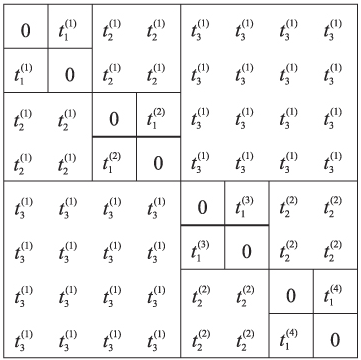
\includegraphics[scale =0.6]{img/matrix.png}\\
  \caption{Parisi matrix in a three step RSB}\label{}
\end{figure}

He then wrote the free energy functional as a function of three invariants of the Parisi matrix, that are
\begin{itemize}

\item{ $q_{\alpha\beta} q_{\beta\alpha} = \Tr q^2$}
\item{ $q_{\alpha\beta} q_{\beta\gamma} q_{\gamma\delta}q_{\delta\alpha} =  \Tr q^4$ }
\item{ $q_{\alpha\beta} q_{\beta\gamma} q_{\gamma\alpha}$ }

\end{itemize}

We remember that the third invariant is not $\Tr q^3$.
Using this particular choice of the matrix, Parisi has been able to evaluate these three invariants in an analytical way, arriving to a non trivial form for $q(x)$ in the $n\rightarrow 0 $ limit.

\section{A connection between two extremals}

The SK model turns out to be a good starting point for the investigation of more complicated models. Obtaining a solution for finite connectivity models (whose EA model is an excellent example) is indeed very complicated.

Let's now proceed in the definition of a somehow intermediate model. A sharp reader will note that the choice of the upcoming model is not casual. 

%\begin{quotation}

%- I'm searching the keys I've lost to get back home.\newline
%- Did you lost them here?\newline
%- No, honestly I do not have idea of where I lost'em..\newline
%- And why are you searching it here?\newline
%- Because, here, there is a light.\newline

%\end{quotation}

\newline
\begin{definition}

A Cayley tree with coordination number $K$ is an infinite connected cycle-free graph where each node is connected to $K+1$ neighbors.

\end{definition}


\begin{figure}[h]
\noindent
		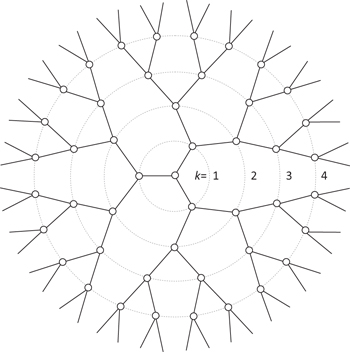
\includegraphics[scale =0.7]{img/cayley.jpg}
	\caption{Cayley tree with coordination number 2}
	\label{fig:cayley}
\end{figure}


Due to the limited number of neighbors, an exact solution of a spin glass defined on this lattice is not a mean field solution.
However in a Cayley tree there are no closed loops, and we will see later that this feature will allow us to derive a simple iterative scheme that will be used to obtain a solution.


\subsection{Boundaries of Cayley tree}

It is easy to check that the number of sites on the boundaries is a finite fraction even in the $N \rightarrow \infty$. The number of sites in the k-th shell $n_j$ can be written as a function of $n_{j-1}$.

\begin{eqnarray}
n_{j} &=& Kn_{j-1} \nonumber\\
      &=& K^2n_{j-2} \nonumber\\
		&=& ... \nonumber\\
		&=& K^{j-1}n_1 \nonumber\\
		&=& K^{j-1}(K+1) \nonumber\\
\end{eqnarray}

Thus the fraction of sites on the boundaries can be evaluated as

\begin{eqnarray}
\lim_{j\rightarrow\infty} \frac{n_{j}}{\sum_{j'=0}^{j-1} n_{j'}}
\end{eqnarray}

This fraction is evaluated in appendix A.
Since the number of boundary sites is relevant in the large N limit, it is preferable to
define our model in a subset of the Cayley tree.

\begin{definition}

A Bethe lattice of a Cayley tree with $L$ shells
is obtained considering only the first
$L'$ shells, where $L'/L \rightarrow 0$

\end{definition}

We empathize that Bethe lattice has no closed loops.

It is important to note that even with this definition, the effect of the
boundary sites is not negligible. In order to eliminate completely the
dependence of the model from the boundary conditions we define the Bethe lattice
as a random graph with fixed connectivity.

\begin{definition}

A random graph with fixed connectivity $K$ is a graph with exactly $K$ links for each node, with each link connecting two random nodes.

\end{definition}

A finite size random graph has closed
loops with length proportional to $\log N$, thus in the thermodynamic limit
the two models are locally equivalent. We will jump from the Bethe lattice to the random graph and viceversa,
depending on what is the most convenient to use in each particular tractation. As an example, when one performs a computer simulation the random graph turns out to be more convenient. However, when we will explain the analytical formulation of the solutions we will use the original Bethe lattice instead.

\begin{figure}[h]
\centering
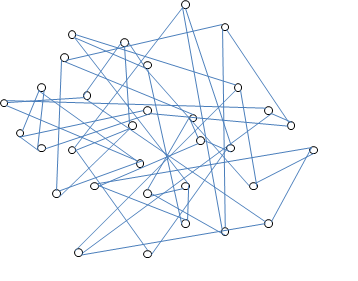
\includegraphics{img/randomgraph.png}
\caption{Random graph, in the large N limit equivalent to Bethe lattice}
\label{fig:}
\end{figure}
